\hypertarget{Distributions_8h}{
\section{Distributions.h File Reference}
\label{Distributions_8h}\index{Distributions.h@{Distributions.h}}
}


This graph shows which files directly or indirectly include this file:\begin{figure}[H]
\begin{center}
\leavevmode
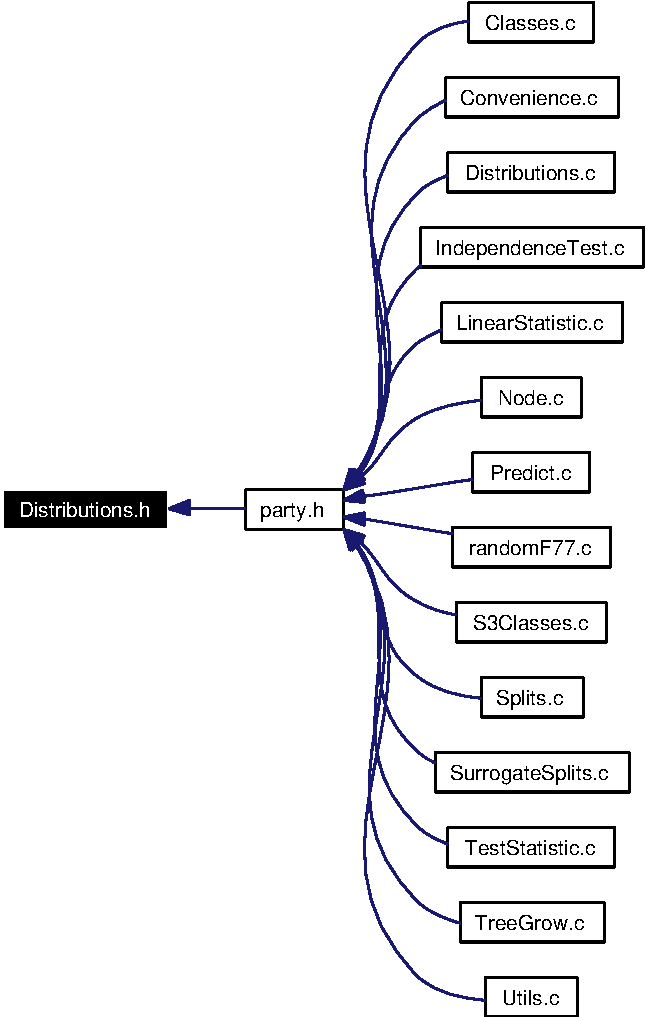
\includegraphics[width=172pt]{Distributions_8h__dep__incl}
\end{center}
\end{figure}
\subsection*{Functions}
\begin{CompactItemize}
\item 
double \hyperlink{Distributions_8h_a692392488ab88e95a62d2142e9d428c}{C\_\-quadform\-Conditional\-Pvalue} (const double tstat, const double df)
\item 
double \hyperlink{Distributions_8h_0b0373aa22dcf8b8ecf6b9c560db9c70}{C\_\-maxabs\-Conditional\-Pvalue} (const double tstat, const double $\ast$Sigma, const int pq, int $\ast$maxpts, double $\ast$releps, double $\ast$abseps, double $\ast$tol)
\item 
void \hyperlink{Distributions_8h_579a9b99cc4ab820a62f636869788cf8}{C\_\-Monte\-Carlo} (double $\ast$pvalues, SEXP learnsample, SEXP weights, SEXP fitmem, SEXP varctrl, SEXP gtctrl, double $\ast$ans)
\end{CompactItemize}


\subsection{Function Documentation}
\hypertarget{Distributions_8h_0b0373aa22dcf8b8ecf6b9c560db9c70}{
\index{Distributions.h@{Distributions.h}!C_maxabsConditionalPvalue@{C\_\-maxabsConditionalPvalue}}
\index{C_maxabsConditionalPvalue@{C\_\-maxabsConditionalPvalue}!Distributions.h@{Distributions.h}}
\subsubsection[C\_\-maxabsConditionalPvalue]{\setlength{\rightskip}{0pt plus 5cm}double C\_\-maxabs\-Conditional\-Pvalue (const double {\em tstat}, const double $\ast$ {\em Sigma}, const int {\em pq}, int $\ast$ {\em maxpts}, double $\ast$ {\em releps}, double $\ast$ {\em abseps}, double $\ast$ {\em tol})}}
\label{Distributions_8h_0b0373aa22dcf8b8ecf6b9c560db9c70}


Conditional asymptotic P-value of a maxabs-type test statistic\par
 Basically the functionality from package `mvtnorm' \par
 \begin{Desc}
\item[Parameters:]
\begin{description}
\item[{\em tstat}]test statitstic \item[{\em Sigma}]covariance matrix \item[{\em pq}]nrow(Sigma) \item[{\em maxpts}]number of Monte-Carlo steps \item[{\em releps}]relative error \item[{\em abseps}]absolute error \item[{\em tol}]tolerance \end{description}
\end{Desc}


Definition at line 52 of file Distributions.c.

Referenced by C\_\-Conditional\-Pvalue(), and R\_\-maxabs\-Conditional\-Pvalue().\hypertarget{Distributions_8h_579a9b99cc4ab820a62f636869788cf8}{
\index{Distributions.h@{Distributions.h}!C_MonteCarlo@{C\_\-MonteCarlo}}
\index{C_MonteCarlo@{C\_\-MonteCarlo}!Distributions.h@{Distributions.h}}
\subsubsection[C\_\-MonteCarlo]{\setlength{\rightskip}{0pt plus 5cm}void C\_\-Monte\-Carlo (double $\ast$ {\em criterion}, SEXP {\em learnsample}, SEXP {\em weights}, SEXP {\em fitmem}, SEXP {\em varctrl}, SEXP {\em gtctrl}, double $\ast$ {\em ans\_\-pvalues})}}
\label{Distributions_8h_579a9b99cc4ab820a62f636869788cf8}


Monte-Carlo approximation to the conditional pvalues \begin{Desc}
\item[Parameters:]
\begin{description}
\item[{\em criterion}]vector of node criteria for each input \item[{\em learnsample}]an object of class `Learning\-Sample' \item[{\em weights}]case weights \item[{\em fitmem}]an object of class `Tree\-Fit\-Memory' \item[{\em varctrl}]an object of class `Variable\-Control' \item[{\em gtctrl}]an object of class `Global\-Test\-Control' \item[{\em ans\_\-pvalues}]return values; vector of adjusted pvalues \end{description}
\end{Desc}


Definition at line 169 of file Distributions.c.

References get\_\-jointtransf(), get\_\-ninputs(), get\_\-nobs(), get\_\-nresample(), PL2\_\-expcovinf\-Sym, PL2\_\-inputs\-Sym, PL2\_\-responses\-Sym, and PL2\_\-sumweights\-Sym.

Referenced by R\_\-Monte\-Carlo().

Here is the call graph for this function:\begin{figure}[H]
\begin{center}
\leavevmode
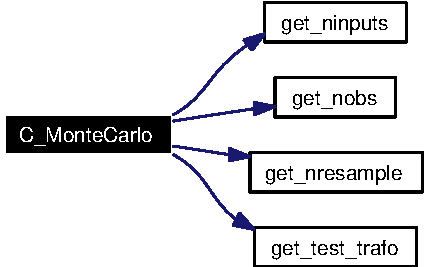
\includegraphics[width=119pt]{Distributions_8h_579a9b99cc4ab820a62f636869788cf8_cgraph}
\end{center}
\end{figure}
\hypertarget{Distributions_8h_a692392488ab88e95a62d2142e9d428c}{
\index{Distributions.h@{Distributions.h}!C_quadformConditionalPvalue@{C\_\-quadformConditionalPvalue}}
\index{C_quadformConditionalPvalue@{C\_\-quadformConditionalPvalue}!Distributions.h@{Distributions.h}}
\subsubsection[C\_\-quadformConditionalPvalue]{\setlength{\rightskip}{0pt plus 5cm}double C\_\-quadform\-Conditional\-Pvalue (const double {\em tstat}, const double {\em df})}}
\label{Distributions_8h_a692392488ab88e95a62d2142e9d428c}


Conditional asymptotic P-value of a quadratic form\par
 \begin{Desc}
\item[Parameters:]
\begin{description}
\item[{\em tstat}]test statistic \item[{\em df}]degree of freedom \end{description}
\end{Desc}


Definition at line 18 of file Distributions.c.

Referenced by C\_\-Conditional\-Pvalue(), and R\_\-quadform\-Conditional\-Pvalue().